\begin{document}
%%%% Liikennesuunnitelmat

\hrule $\color{white}{.}$ \\
Merkitään 
\begin{itemize}
    \item $\mathcal{B}$ Borelin $\sigma$-algebra joukossa $K$
    \item $\Omega = [0,|\Omega|]$, kaikkien säikeiden indeksijoukko. (Kirjan johdannossa valittu [0,1])
    \item $X$ kompakti, konveksi $R^n$ osajoukko, $X \subset R^n$.
    \item $|A|$ Mitallisen joukon $A\subset \R$ Lebesgue-mitta.
    \item $K$ Merkitään kaikkien 1-Lipschitz kuvauksien $\gamma:\R^+ \to X$ joukkoa $K$. 
    \item $\mathcal{P}(E)$ joukon $E$ osajoukkojen kokoelmaa, VAIHDA
\end{itemize}
\hrule


\begin{definition}
    Määritellään etäisyys joukossa $K$ siten, että
    \[d(\gamma, \gamma') = \sup_k \frac{1}{k}||\gamma - \gamma||_{L^\infty([0,k])}\]
\end{definition}

\begin{definition}
    Määritellään polun $\gamma \in K$ pysähtymisajaksi 
    \begin{equation*}
        T(\gamma) = \inf\{t\ge0:\gamma \text{ vakio välillä } [t,\infty[ \}
    \end{equation*}
    ja pituudeksi $L(\gamma)$ polun pituus välillä $[0, T(\gamma)]$ eli
     \begin{equation*}
         L(\gamma) = \int_0^{T(\gamma)}|\gamma'(t)|\, \dt.
     \end{equation*}
\end{definition}

Polun pysähtymisaika kuvastaa sitä, mistä parametrin arvosta $t$ lähtien polun $\gamma$ pisteet pysyvät paikallaan. On järkevää rajoittaa tarkastelu sellaisiin polkuihin, jotka päättyvät jossakin kohtaa.

\begin{definition}\label{def:liikennesuunnitelma}
    Mitta $\P: K \to \R^+$ avaruudessa  $(K, \Borel)$ on \textbf{liikennesuunnitelma}, jos
    \begin{equation*}
     \int_K T(\gamma) \, \d \P (\gamma) < \infty.   
    \end{equation*}
\end{definition}

Liikennesuunnitelman määritelmä sallii, että $\P$-nollamittainen joukko polkuja $\gamma$ on pituudeltaan äärettömiä, eli joille $T(\gamma) = \infty$.

\begin{definition}
    Olkoon $\P$ liikennesuunnitelma. Merkitään joukon $X$ kaikkia liikennesuunnitelmia $TP = TP(X)$, ja $TP_C = TP_C(X)$ kaikkia joukon $X$ liikennesuunitelmia $\P$ joille
    \begin{equation*}
        \int_K T(\gamma) \d \P(\gamma) \le C.
    \end{equation*}
\end{definition}

\begin{definition}
    Olkoon $\pi_0, \pi_\infty: K\to X$ ja $\pi:K\to X \times X$ kuvauksia, jotka määritellään polulle $\gamma \in K$ siten, että 
    \begin{align*}
        \pi_0(\gamma) &= \gamma(0) &&\Big| \text{ Polun lähtöpiste. }\\
        \pi_\infty(\gamma) &= \gamma(T(\gamma)) &&\Big| \text{ Polun päätepiste. }\\
        \pi(\gamma) &= (\gamma(0), \gamma(T(\gamma)) &&\Big| \text{ Polun lähtöpiste ja päätepiste. }
    \end{align*}
\end{definition}

\begin{definition}
    Olkoon $\P$ liikennesuunnitelma. Määritellään mitat $\mu^+, \mu^- : X \to \mathbf{R}_+$ ja $\pi: X\times X \to \mathbf{R}_+$ siten, että
    \begin{align*}
        \mu^+(\P) &= \pi_{0\#} \P  &&\Big| \text{ Irrigoiva mitta, \textit{irrigating measure} }\\
        \mu^-(\P) &= \pi_{\infty \#} \P  &&\Big| \text{ Irrigoitu mitta, \textit{irrigating measure} }\\
        \pi(\P) &= \pi_\# \P  &&\Big| \text{ Siirtosuunnitelma liikennesuunnitelmalle $\P$,}\\ 
        & &&\hphantom{\Big|} \text{ \textit{transference plan of $\P$}}
    \end{align*}
\end{definition}

\begin{figure}
    \centering
    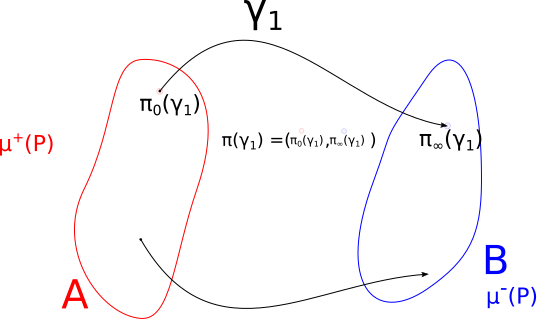
\includegraphics[scale=0.8]{graphics/irrigoiva-ja-irrigoitu-mitta.png}
    \caption{Havainnollistus sovituista merkinnöistä.\todo{Merkittävä mitan $\mu^+$ support}, eli joukko, missä mitta saa aidosti positiivisia arvoja.}
    \label{fig:my_label}
\end{figure}


\begin{remark}
    Kaikille Borelin joukoille $A, B \subset K$ pätee
    \begin{align*}
        \mu^+(\P)(A) &= \P(\pi_0^{-1}(A)) = \P(\{\gamma \in K : \gamma(0) \in A\}) \\
        \mu^-(\P)(B) &= \P(\pi_\infty^{-1}(B)) = \P(\{\gamma \in K : \gamma(\infty) \in B\}) \\
        \pi(\P)(A\times B) &= \P(\pi(A\times B)) = \P(\{\gamma \in K: \gamma(0) \in A\text{ ja } \gamma(\infty) \in B)\}
    \end{align*}
\end{remark}

Liikennesuunnitelman irrigoiva mitta on mitta sille joukolle, mistä massaa ollaan lähettämässä ja irrigoitu mitta mihin sitä ollaan lähettämässä. Liikennesuunnitelman siirtosuunnitelma sisältää tiedon siitä, minne minkäkin pisteen massa lähetetään.

\subsection{Parametrisoidut liikennesuunnitelmat}
 
\begin{theorem}\label{thm:skorohkod}
    Olkoon $\P: K \to \R^+$ liikennesuunnitelma. Tällöin on olemassa mitallinen funktio $\chi: [0, c] \to K$ siten, että liikennesuunnitelma voidaan kirjoittaa muodossa $$\P =\chi_\# \lambda.$$
\end{theorem}
\begin{proof}
    Lause seuraa Skorohkodin lauseesta, joka on todistettu lähteessä \cite[p. 185]{OptimalTransportationNetworks}.
\end{proof}
Edellisen lauseen mukaan mikä tahansa liikennesuunnitelma $\P$ voidaan parametrisoida mitallisella funktiolla $ \chi: [0, c] \to K$ s. e. $\P = \chi_\# \lambda$, missä $\lambda$ on Lebesguen mitta välille $[0,c]$. 

Funktio $ \chi:[0, c] \to K$ antaa siis jokaiselle välin $[0, c]$ luvulle 1-Lipschitz-polun joukosta $K$. 
Merkitään jatkossa $\Omega = [0,c]$ ja kutsutaan väliä indeksijoukoksi. Polku $ \chi(\omega)$ vastaa siis indeksin $\omega$ hiukkasen reittiä.

Merkitään nyt $\chi(\omega, t) :=  \chi(\omega)(t)$ kaikille $\omega \in \Omega$ ja $t \in \R^+$. Jatkossa, kun käytetään merkintää $\chi(\omega, t)$, tarkoitetaan funktiota $\chi : \Omega \times \R^+ \to X$. Osoitetaan seuraavaksi, että myös näin määriteltynä $\chi$ on mitallinen funktio.

\begin{theorem}
    Funktio $\chi: \Omega \times \R^+ \to X $ on mitallinen jos funktio $ \chi: \Omega \to K$ on mitallinen.
\end{theorem}
\begin{proof}
Bernot, Caselles: Optimal transportation networks s.27 (joss.-versio)
\end{proof}
Funktion $\chi$ pysähdysaika määritellään vastaavasti, kuten liikennesuunnitelman $\P$ pysähdysaika.
\begin{definition}
    Jos $\chi: \Omega \times \R^+ \to X$ on mitallinen, niin sen \textit{pysähdysaika} $T_\chi$ on
    \[T_\chi (\omega) = \inf\{t : \chi(\omega, t) \text{ on vakio välillä } [t,\infty[\}.\]
\end{definition}

Määritellään seuraavaksi, milloin liikennesuunnitelman $\P$ parametrisaatio $\chi$ on myös liikennesuunnitelma.
\begin{definition} \label{def:parameterizedTP}
    Olkoon $\Omega \subset \R$ Lebesgue-mitallinen ja Lebesgue-mitaltaan äärellismittainen. Mitallinen kuvaus $\chi: \Omega \times \R^+ \to X$ on \textbf{parametrisoitu liikennesuunnitelma}, jos $t\to \chi(w,t)$ on 1-Lipschitz kaikille $\omega \in \Omega$ ja
    \[\int_\Omega T_\chi (\omega) \, \d \omega < \infty .\]
\end{definition}

Eritellään vielä käyttöön otetut merkinnät ja nimetään ne.
\begin{definition}
    Olkoon $\Omega\subset \R$ mitallinen ja äärellismittainen. Olkoon lisäksi $\chi$ liikennesuunnitelman $\P$ parametrisoitu liikennesuunnitelma.
    \begin{itemize}
        \item Funktio $\chi:\Omega \times \R^+ \to X$ on parametrisoitu liikennesuunnitelma. 
        \item Polku $\chi(\omega, \cdot)$ on \textit{säie}.
        \item Polun $\chi(\omega, \cdot)$ kuvajoukko on myös \textit{säie}.
    \end{itemize}
\end{definition}

\begin{theorem}\label{thm:push-cov}
    Olkoon Borelin avaruudet $(X_1, \Sigma_1)$ ja $(X_2, \Sigma_2)$, mitallinen kuvaus $f: X_1 \to X_2$, mitta $\mu:\Sigma_1 \to [0, \infty]$\what{ja $g: X_2 \to \R^+$ integroituva}. Tällöin
    
    \begin{equation*}
        \int_{X_2} g \, d(f_{\#} \mu) = \int_{X_1} g \circ f \, d\mu.
    \end{equation*}
\end{theorem}
\begin{proof}
LÄHDE?
\end{proof}

\begin{theorem}
    Olkoon $\chi : \Omega \times \R^+ \to X$ parametrisoitu liikennesuunnitelma.
    Määritellään mitta $\P_\chi : K \to \Omega$ siten, että \[\P_\chi (E) = \lambda(\chi^{-1}(E)) = \chi_\#\lambda\] jokaiselle Borelin joukolle $E\subset K$. 
    Tällöin $\P_\chi$ on \textit{liikennesuunnitelma}. 
\end{theorem}

\begin{proof}
Osoitetaan, että $\P_\chi$ toteuttaa Määritelmän \ref{def:liikennesuunnitelma}.
\begin{align*}
    \int_K T(\gamma)\, d\P_\chi(\gamma) = &\int_K T(\chi(\omega))\, d\P_\chi(\chi(\omega)) \\
    =& \int_K T_\chi(\omega) \, d(\chi_\# \lambda(\omega)) \\
    \stackrel{\ref{thm:push-cov}}{=}& \int_\Omega T_\chi(\omega)(\chi) \, d\lambda(\omega) \\
    =& \int_\Omega T_\chi(\omega)(\chi) \, d\omega \stackrel{\ref{def:parameterizedTP}}{<} \infty.
\end{align*}

\end{proof}



\subsection{Liikennesuunnitelmien {stabiliteetti}}


\begin{definition}
    Olkoon funktio $f:A \to \R$, missä $A\subset \R^n$. Funktion $f$ kantaja $\supp(f)$ on funktion $f$ määrittelyjoukon osajoukko, jossa funktio $f$ saa nollasta poikkeavia arvoja, eli
    \begin{equation*}
        \supp(f) = \{x \in X | f(x) \ne 0\}.
    \end{equation*}
\end{definition}

\begin{definition}
    Olkoon funktio $f: A \to \R$, missä $A\subset \R^n$ Jos funktio $f$ on jatkuva joukossa $A$, niin merkitään $f \in C(A)$ tai $f \in C(A, \R)$. Jos lisäksi funktion $f$ kantaja on kompakti, merkitään $f \in C_c(A)$.
\end{definition}

\begin{definition} \label{def:weakConv}
    Olkoon $\P \in \mathcal{P}(X)$ liikennesuunnitelma metrisessä avaruudessa $(X, d)$. Liikennesuunnitelmien $\P_n \in \mathcal{P}(X)$ jono $(\P_n)$ suppenee heikosti, merkitään $\P_n \rightharpoonup \P$, jos pätee 
    \begin{equation*}
        \lim_{n\to\infty} \int_X f(x) \, d\P_n (x) = \int_X f(x) \, d\P(x)
    \end{equation*}
    kaikilla $f \in C_c(X)$.
\end{definition}

\begin{definition}
    Olkoon $\P_n$ jono liikennesuunnitelmia. Sanotaan, että jono $\P_n$ suppenee kohti liikennesuunnitelmaa $\P$, jos 
    $$\P_n \rightharpoonup \P \, \text{ tai}$$
    $$ \chi_n (\omega) \to  \chi (\omega) \text{ joukossa } K \text{ melkein kaikille } \omega
    \in \Omega,$$
    missä $ \chi_n$ ja $ \chi$ ovat Lauseen \ref{thm:skorohkod} mitalliset funktiot liikennesuunnitelmille $\P_n$ ja $\P$ vastaavassa järjestyksessä.
\end{definition}

\subsubsection{Pituuden, pysähdysajan, keskipituuden ja keskipysähdymisajan alhaalta puolijatkuvuus}

\begin{lemma}\label{le:LSCisLimitOfC-Functions}
    Jokainen alhaalta puolijatkuva funktio $f$ kompaktissa metrisessä avaruudessa on jatkuvien funktioiden kasvavan jonon raja-arvo.
\end{lemma}

\begin{proof}
    Todistus mukailee todistusta \cite[p. 30]{OptimalTransportationNetworks}. Olkoon $f:\R^n \to \R$ alhaalta puolijatkuva. Asetetaan $\displaystyle f_k(x) := \inf_y\{f(y) + kd(x,y)\}$. Tällöin $f_k$ on \whytho{jatkuva}. Lisäksi \whytho{$f_1 \le f_2 \le ... \le f$}.
    Olkoon $\varepsilon > 0$. Oletetaan, että $f \ge 0$. Koska $f$ on alhaalta puolijatkuva, on olemassa $\delta > 0$ siten, että $f(y) > f(x) - \varepsilon$ kaikilla $y \in B(x, \delta).$ ... (\url{https://math.stackexchange.com/questions/165764/lower-semicontinuous-function-as-the-limit-of-an-increasing-sequence-of-continuo})
\end{proof}

\begin{lemma}\label{le:fdPLeLiminf}
    Olkoon $(\P_n)$ jono positiivisia mittoja kompaktissa metrisessä avaruudessa $K$ siten, että $\P_n \rightharpoonup \P$. Olkoon $\gamma \mapsto f(\gamma)$ alhaalta puolijatkuva funktio avaruudessa $K$. Tällöin
    \begin{equation*}
        \int_K f(\gamma) \, d\P(\gamma) \le \liminf_n \int_K f(\gamma) \, d\P_n(\gamma).
    \end{equation*}
\end{lemma}

\begin{lemma}\label{le:pysahtymisajan&pituudenLSC}
    Olkoon jono polkuja $\gamma_n \in K$ Jos jono $(\gamma_n)$ suppenee polkuun $\gamma \in K$ etäisyyden $d$ suhteen, niin
    \begin{equation*}
        T(\gamma) \le \liminf_n T(\gamma_n),
    \end{equation*}
    ja 
    \begin{equation*}
        L(\gamma) \le \liminf_n L(\gamma_n).
    \end{equation*}
\end{lemma}

\begin{lemma}
    Jos jono liikennesuunnitelmia $\P_n$ suppenee liikennesuunnitelmaan $\P$, niin 
    \begin{equation*}
        \int_K T(\gamma) \, d\P(\gamma) \le \liminf_n \int_K T(\gamma) \, d\P_n(\gamma),
    \end{equation*}
    ja
    \begin{equation*}
        \int_K L(\gamma) \, d\P(\gamma) \le \liminf_n \int_K L(\gamma) \, d\P_n(\gamma).
    \end{equation*}
\end{lemma}

\subsection{Liikennesuunnitelman kertaluku ja liikennesuunnitelman ylhäältä puolijatkuvuus}

\begin{definition}
Olkoon $\chi : \Omega \times \R^+ \to X$ liikennesuunnitelman $\P$ parametrisaatio. Määritellään polkuluokka alkiolle $x\in \R^n$ liikennesuunnitelmassa $\chi$ joukkona
\begin{equation*}
    \Omega_x^\chi = \{\omega : x \in \chi(\omega, \R)\}.
\end{equation*}
ja alkion $x$ kertaluvuksi
    \begin{equation*}
        |x|_\chi = |\Omega_x^\chi| = |\P(\{\gamma : \exists t, \gamma(t) = x\}) = |x|_\P.
    \end{equation*}
\end{definition}

Alkion $x\in \R^n$ polkuluokka sisältää ne kaikki säikeiden $\chi$ indeksit $\omega$, jotka kulkevat alkion $x$ kautta. Kertaluku kuvastaa taas sitä, kuinka useasti säie $\chi$ kulkee alkion $x$ kautta.

\begin{theorem} \label{thm:multiplicityXnLeX}
    Olkoon $(\chi_n)$ jono liikennesuunnitelmia, jotka suppenevat liikennesuunnitelmaan $\chi$. Oletetaan, että $\int_\Omega T(\chi_n(\omega))\, d\omega \le C$ jollekin $C$. Tällöin melkein-kaikille $\omega$ pätee
    \begin{equation*}
        \limsup |\chi_n(\omega, t)|_{\chi_n} \le |\chi(\omega, t)|_\chi.
    \end{equation*}
\end{theorem}
\begin{proof}
    Todistus mukailee todistusta \cite[p. 31-32]{OptimalTransportationNetworks}. Merkitään $[x]_\chi := \Omega_x^\chi$, eli alkion $x\in \R^n$ polkuluokkaa $[x]_\chi$. Olkoon $M > 0.$ Markovin epäyhtälön \ref{thm:markov} nojalla saadaan
    \begin{equation*}
        |\{\omega : T(\chi_n(\omega)) > M\}| \le \frac{C}{M|\Omega|} =: \varepsilon.
    \end{equation*}
    Määritellään approksimatiivinen kertaluku
    \begin{equation*}
        [\chi(\omega,t)]_\chi^\varepsilon := \left\{\omega' \in [\chi(\omega, t)]_\chi : T(\chi(\omega')) \le M = \frac{\varepsilon|\Omega|}{C}\right\}.
    \end{equation*}
    Olkoon $\omega' \in \cap_k \cup_{n > k} [\chi_n(\omega, t)]_{\chi_n}$. Tällöin on olemassa jono  indeksejä $n_i$ joka lähestyy ääretöntä, ja ajat $s_i$ joille $\chi_{n_i}(\omega',s_i) = \chi_{n_i}(\omega, t)$. Toisin sanoen, koska $\omega'$ kuuluu samaan polkuluokkaan kuin $\omega$, löydetään ajanhetkelle $t$ ajanhetki $s_i$ siten, että $\chi_{n_i}(\omega',s_i) = \chi_{n_i}(\omega, t)$. Koska $s_i\le T(\chi_{n_i}(\omega) \le M$ on $(s_i)$ rajoitettu jono, on olemassa suppeneva osajono, joka suppenee johonkin $s$. Koska $(\chi_{n_i}(\omega', \cdot))$ on jono 1-Lipschitz-polkuja kompaktilla välillä $[0, M]$, niin se suppenee tasaisesti välillä $[0, M]$, jolloin saadaan $\chi(\omega', s) = \chi(\omega, t)$, koska $\omega' \in [\chi(\omega, t)]_\chi$. Tämä osoittaa sen, että 
    \begin{equation*}
        \cap_k \cup_{n > k} [\chi_n(\omega, t)]_{\chi_n}^\varepsilon \subset [\chi(\omega, t)]_\chi,
    \end{equation*}
    \what{joten}
    %TR: Tuosta inkluusiosta seuraa epäyhtälö esimerkiksi monotonisen konvergenssin kautta (indikaattorifunktioille). Limsup tuosta mitasta on pienempää kuin lim k\to\infty yhdisteen n \ge k mitasta. Tämä jälkimmäinen jono on monotoninen, ja edellisen inkluusion nojalla lim tuon joukon karakterisesta funktiosta on korkeintaan inkluusion oikeanpuoleisen joukon karakterinen funktio. Viimeisessä epäyhtälössä käytetään sitä tietoa, että varsinaisessa kertaluvussa mitataan lisäksi polkuja jotka ovat tuossa korkeintaan epsilon-mittaisessa poikkeusjoukossa (johon siis tungettiin kaikki liian pitkät polut). Mitaltaan siis tuo approximatiivinen ja varsinainen joukko poikkeavat korkeintaan tuon epsilonin verran.
    \begin{equation*}
        \limsup_n |[\chi_n(\omega, t)]_{\chi_n}^\varepsilon| \le |[\chi(\omega, t)]_\chi|.
    \end{equation*}
    Siispä
    \begin{equation*}
        \limsup_n |[\chi_n(\omega, t)_{\chi_n}]| - \varepsilon \le |[\chi(\omega, t)]_\chi|.
    \end{equation*}
\end{proof}
\begin{lemma}\label{le:multiplicityUSC}
    Olkoon $\chi$ parametrisaatio liikennesuunnitelmalle $\P$. Tällöin funktio $x \mapsto |x|_\chi$ on ylhäältä puolijatkuva.
\end{lemma}
\begin{proof}
    \textbf{Ei käytössä.}
    Todistus mukailee lähdettä \cite[p. 32]{OptimalTransportationNetworks}. Merkitään $\phi: x \to |x|_\chi$. Osoitetaan, että jokaiselle $x$, jolle $|x|_\chi < r$, on olemassa pallo $B(x, \varepsilon)$ siten, että kaikille $y \in B(x, \varepsilon)$ pätee $|y|_\chi < r$. Tämä osoittaa, että $\phi^{-1}([0, r[)$ on avoin joukko, josta \what{seuraa} funktion $\phi$ ylhäältä puolijatkuvuus. Osoitetaan väite käänteisellä päättelyllä, olettaen, että $\phi^{-1}([0, r[)$ ei ole avoin. Tällöin pallossa $B(x, \frac{1}{n})$ on olemassa $y_n \in B(x, \frac{1}{n})$, jolle $|y_n|_\chi \ge r$ kaikilla $n\in \N$. Selvästi $\lim_{n\to\infty} y_n = x$. Olkoon
    \begin{equation*}
        \tilde{\Omega} = \bigcap_m \bigcup_{n \ge m} \Omega_{y_n}^\chi.
    \end{equation*}
    Poistamalla tarvittaessa nollamittainen joukko, saadaan $\tilde{\Omega} \subset \Omega_x^\chi$. Jos $\omega \in \tilde{\Omega}$, niin kaikille $m$ on olemassa $n \ge m$ siten, että $\omega \in \Omega_{y_n}^\chi$. Tällöin on olemassa $t_n$ jolle $\chi(\omega, t_n) = y_n$. 
    Koska melkein kaikille $\omega$ pätee $T(\chi(\omega)) < \infty$, jonon $(t_n)$ voidaan olettaa rajoitetuksi. Tällöin on olemassa jonon $(t_n)$ osajono $(t_{n_k})$ jolle $t_{n_k} \to t$ siten, että $\chi(\omega, t) = x$, eli $\omega \in \Omega_x^\chi$. Siispä $|\tilde{\Omega}| \ge |x|_\chi < r$ ja $|\tilde{\omega}| = \lim_m |\bigcup_{n \ge m} \Omega_{y_n} \ge r$.
\end{proof}

\begin{corollary}
    Olkoon $\chi$ parametrisaatio liikennesuunnitelmalle $\P$. Tällöin funktio $(\omega, t) \mapsto |\chi(\omega, t)|_\chi$ on mitallinen.
\end{corollary}

\subsection{Liikennesuunnitelmien jonokompaktisuus}

\begin{theorem}\label{le:tfPlanWeakConv}
    Jos $(\P_n)$ on jono joukossa $TP_C$ siten että $\P_n \rightharpoonup \P$, niin $\pi(\P_n) \rightharpoonup \pi(\P)$. Lisäksi 
    \begin{equation*}
    \mu^+(\P_n) \rightharpoonup \mu^+(\P) \text{ ja }  \mu^-(\P_n) \rightharpoonup \mu^-(\P) 
    \end{equation*}
    
\end{theorem}
\begin{proof}
    Todistus mukailee lähdettä \cite[p. 33]{OptimalTransportationNetworks} Oletetaan, että $\P_n$ on todennäköisyysmitta korvaamalla $\P_n$ mitalla $\frac{\P_n}{\P_n(K)}$. Merkitään $K_\varepsilon := \{\gamma \in K : T(\gamma) \le M\}$. Tällöin
    \begin{align*}
        \P_n(K\setminus K_\varepsilon) &= \P_n(K\setminus\{\gamma \in K: T(\gamma) \le M\} \\
        &= \P_n(\{\gamma \in K : T(\gamma) > M\}).
    \end{align*}
    Markovin epäyhtälöllä \ref{thm:markov} ja tiedolla $\P_n \in TP_C$ saadaan 
    \begin{equation*}
        \P_n(\{\gamma \in K : T(\gamma) > M\}) \le \frac{1}{M}\int_K |T(\gamma)| \, d\P_n \le \frac{C}{M},
    \end{equation*}
    Asetetaan $\varepsilon := \frac{C}{M}$, jolloin
    \begin{equation*}
        \P_n(K\setminus K_\varepsilon) \le \varepsilon.
    \end{equation*}
    Olkoon $\phi \in C(X\times X, \R)$. Osoitetaan, että tällöin funktio $\gamma \mapsto \phi(\gamma(0), \gamma(M))$ on jatkuva. Koska $\phi$ on jatkuva, riittää osoittaa, että funktio $F: K\to X \times X : \gamma \mapsto (\gamma(0), \gamma(M))$ on jatkuva. Olkoon $\gamma_1, \gamma_2 \in K$. Koska
    \begin{equation*}
        d(\gamma_1, \gamma_2) = \sup_{k\in\N} \frac{1}{k}||\gamma_1-\gamma_2||_{L^\infty([0,k])}
    \end{equation*}
    niin tällöin
    \begin{align*}
        d_X(\gamma_1(0), \gamma_2(0)) + d_X(\gamma_1(M), \gamma_2(M)) &\le \frac{1}{1}||\gamma_1-\gamma_2||_{L^\infty([0,1])} + M\frac{1}{M}||\gamma_1-\gamma_2||_{L^\infty([0,M])} \\
        &\le  d(\gamma_1, \gamma_2) + Md(\gamma_1, \gamma_2) \\
        &\le (M+1)d(\gamma_1, \gamma_2).
    \end{align*}
    Toisin sanoen, $F$ on $(M+1)$-Lipschitz-jatkuva.
    Siispä $\gamma \mapsto \phi(\gamma(0), \gamma(M))$ on jatkuva. Osoitetaan, että tämä funktio toteuttaa heikon suppenemisen Määritelmän \ref{def:weakConv}. Merkitään $\pi(\P_n) = \pi_{\P_n}$ ja $\pi(\P) = \pi_\P$.  Koska siirtosuunnitelma on määritelty muodossa $\pi_{\P_n} = \pi_\#\P_n$, niin Muuttujanvaihtolauseen \ref{thm:push-cov} nojalla saadaan
    \begin{align*}
        \limsup_{n\to\infty} \int_{X \times X} \phi(x, y) \, d\pi_{\P_n} (x, y) &= \limsup_{n\to\infty} \int_{K} \phi(\pi_{\P_n}(\gamma)) \, d\P_n (\gamma)  
    \end{align*}
    Koska $K = K_\varepsilon \cup K \setminus K_\varepsilon$, niin integraali voidaan paloitella. Saadaan
    \begin{align*}
        \int_{K} \phi(\pi_{\P_n}(\gamma)) \, d\P_n (\gamma) &= \int_{K_\varepsilon} \phi(\pi_{\P_n}(\gamma)) \, d\P_n (\gamma) + \int_{K \setminus K_\varepsilon} \phi(\pi_{\P_n}(\gamma)) \, d\P_n (\gamma) \\
        &\le \int_{K_\varepsilon} \phi(\pi_{\P_n}(\gamma)) \, d\P_n (\gamma) + \P_n(K\setminus K_\varepsilon) ||\phi||_\infty\\
        &\le \int_{K_\varepsilon} \phi(\gamma(0),\gamma(T(\gamma))) \, d\P_n (\gamma) + \varepsilon||\phi||_\infty \\
        &=  \int_{K_\varepsilon} \phi(\gamma(0),\gamma(M)) \, d\P_n (\gamma) + \varepsilon||\phi||_\infty \\
        &\le \int_{K} \phi(\gamma(0),\gamma(M)) \, d\P_n (\gamma) + 2\varepsilon||\phi||_\infty.
    \end{align*}
Siispä 
    \begin{align} \label{eq:tfWeakConv2}
        \limsup_{n} \int_{K} \phi(\pi_{\P_n}(\gamma)) \, d\P_n (\gamma) \le \limsup_n \int_{K} \phi(\gamma(0),\gamma(M)) \, d\P_n (\gamma) + 2\varepsilon||\phi||_\infty.
    \end{align}
Koska $\P_n \rightharpoonup \P$ ja $\gamma \mapsto \phi(\gamma(0), \gamma(M))$ on jatkuva, niin 
    \begin{equation*}
        \limsup_n \int_{K} \phi(\gamma(0),\gamma(M)) \, d\P_n (\gamma) = \int_{K} \phi(\gamma(0),\gamma(M)) \, d\P (\gamma),
    \end{equation*}
jolloin epäyhtälö \eqref{eq:tfWeakConv2} saadaan muotoon
    \begin{align*}
        \limsup_{n} \int_{K} \phi(\pi_{\P_n}(\gamma)) \, d\P_n (\gamma) \le \int_{K} \phi(\gamma(0),\gamma(M)) \, d\P (\gamma) + 2\varepsilon||\phi||_\infty.
    \end{align*}
Lisäksi saadaan
    \begin{align*}
        \int_K \phi(\gamma(0),\gamma(M)) \, d\P (\gamma) &\le \int_{K_\varepsilon} \phi(\gamma(0),\gamma(M)) \, d\P (\gamma) + \varepsilon||\phi||_\infty \\
        &=\int_{K_\varepsilon} \phi(\gamma(0),\gamma(T(\gamma))) \, d\P (\gamma) + \varepsilon||\phi||_\infty \\
        &\le \int_{K} \phi(\gamma(0),\gamma(T(\gamma))) \, d\P (\gamma) + 2\varepsilon||\phi||_\infty.
    \end{align*}
Siispä
    \begin{equation*}
        \limsup_{n} \int_{K} \phi(\pi_{\P_n}(\gamma)) \, d\P_n (\gamma) \le \int_{K} \phi(\gamma(0),\gamma(T(\gamma))) \, d\P (\gamma) + 4\varepsilon||\phi||_\infty.
    \end{equation*}
Muuttujanvaihtolauseen \ref{thm:push-cov} mukaan voidaan integraalit korvata siten, että
    \begin{equation*}
        \limsup_{n\to\infty} \int_{X \times X} \phi(x, y) \, d\pi_{\P_n} (x, y) \le \int_{X \times X} \phi(x, y) \, d\pi_{\P} (x, y) + 4\varepsilon||\phi||_\infty.
    \end{equation*}
Vastaavasti voidaan osoittaa, että 
    \begin{equation*}
        \liminf_{n\to\infty} \int_{X \times X} \phi(x, y) \, d\pi_{\P_n} (x, y) \ge \int_{X \times X} \phi(x, y) \, d\pi_{\P} (x, y) - 4\varepsilon||\phi||_\infty.
    \end{equation*}

Koska $\phi$ on mielivaltainen funktio ja $\varepsilon > 0$, niin $\pi_{\P_n} \rightharpoonup \pi_\P$.
\end{proof}

\begin{corollary}
    Olkoon $\pi$ mitta joukossa $X \times X$. Tällöin on olemassa liikennesuunnitelma $\P$ siten, että $\pi_\P = \pi$.
\end{corollary}

\section{Liikennesuunnitelman energia ja sen minimoijan olemassaolo}
 Sovitaan, että $0^{\alpha - 1} = \infty$, kun $\alpha \in [0, 1]$.

\begin{definition}\label{def:energyOfP}
    Olkoon $\alpha \in [0, 1].$ Liikennesuunnitelman $\P$ energia parametrisaatiolla $\chi$ on \define{funktionaali}
        \begin{equation*}
            \E^\alpha(\P) = \int_\Omega \int_{\R^+} |\chi(\omega, t)|_\chi^{\alpha-1}|\dot \chi(\omega, t)|\, dtd\omega.
        \end{equation*}
\end{definition}
    
\begin{remark}\label{thm:energyOfPIndependent}
    Olkoon $\alpha \in [0, 1].$ Liikennesuunnitelman $\P$ energia voidaan kirjoittaa muodossa
    \begin{equation*}
        \E^\alpha(\P) = \int_K \int_{\R^+}|\gamma(t)|^{\alpha-1}_\P|\dot\gamma(t)| \, dtd\P(\gamma).
    \end{equation*}
\end{remark}
\begin{proof}
    Todistetaan muuttujanvaihtolauseella \ref{thm:push-cov}.
\end{proof}

Jatkon kannalta on helpompaa käsitellä liikennesuunnitelmia $\P$, jotka sisältävät vain säikeitä $\chi$, joiden nopeus on yksi, eli $\dot\chi(\omega, t) = 1$ kaikilla $(\omega, t) \in \Omega \times \Rp$. Osoitetaan, että liikennesuunnitelmalle $\P$ löytyy liikennesuunnitelma $\tilde \P$, jonka säikeet on parametrisoitu pituuden mukaan ja sen energia säilyy samana kuin liikennesuunnitelman $\P$.

\begin{lemma}
    Olkoon $\chi : [0, 1] \to K$ liikennesuunnitelman $\P$ parametrisaatio. Olkoon $S:[0,1]\times \Rp \to \Rp$ funktio, jolle $S(\omega, t)$ on 1-Lipschitz-jatkuva ja kasvava kaikilla $t \in \Rp$. Olkoon $\tau:[0, 1] \times [0, \infty [ \to \Rp$ ja määritellään
    \begin{equation*}
        \tau(\omega, s) := \inf \{t \in [0, \infty[ : S(\omega, t)\}.
    \end{equation*}
    Oletetaan, että $\tau$ on mitallinen. Tällöin $\tilde\chi(\omega, t) = \chi(\omega, \tau(\omega, t))$ on mitallinen.
\end{lemma}
\begin{proof}
    Todistus löytyy lähteestä \cite[p.44]{OptimalTransportationNetworks}
\end{proof}

\begin{lemma}\label{le:parametrizedByLength}
    Olkoon $\chi:[0,1] \to K$ liikennesuunnitelman $\P$ parametrisaatio. Olkoon 
    \begin{equation*}
        S(\omega, t) = \int_0^t|\dot\chi(\omega, r)| \, dr,
    \end{equation*}
    ja asetetaan
    \begin{equation*}
        T(\omega, s) = \inf\{t \in [0,\infty[ : S(\omega, t) = s\}.
    \end{equation*} 
    Olkoon $\tilde \chi(\omega, s) = \chi(\omega, T(\omega, s))$. Tällöin $\tilde\chi$ on Lebesgue-mitallinen ja liikennesuunnitelman jokainen säie on parametrisoidu pituuden mukaan. Lisäksi, kun $\tilde \P = \tilde \chi_\# \lambda $, niin $\E^\alpha(\tilde\P) = \E^\alpha(\P)$.
\end{lemma}

\begin{proof}
    Todistus löytyy lähteestä \cite[p.40]{OptimalTransportationNetworks}.
\end{proof}

Edellisessä lemmassa $T$ antaa ensimmäisen ajanhetken, jolloin ollaan kuljettu matka $s$.

\begin{lemma}\label{le:nrgGeThanLength}
    Olkoon $P \in \mathcal{P}(K)$ liikennesuunnitelma. Tällöin
        \begin{equation*}
            \E^\alpha(\P) \ge \int_K L(\gamma) \, d\P(\gamma).
        \end{equation*}
\end{lemma}

\begin{proof}
    Todistus mukailee todistusta \cite[p. 36]{OptimalTransportationNetworks}. Lauseen \ref{thm:energyOfPIndependent} nojalla energia voidaan kirjoittaa muodossa
    \begin{equation*}
        \E^\alpha(\P) = \int_K \int_{\R^+}|\gamma(t)|^{\alpha-1}_\P|\dot\gamma(t)| \, dtd\P(\gamma).
    \end{equation*}
     Koska liikennesuunnitelman $\P$ massa on 1, niin kaikkien pisteiden $x \in \R^n$ kertaluku on oltava pienempää kuin 1, eli  $|x|_\P \le 1$. Koska $\alpha \in [0, 1]$, niin  $|x|^{\alpha-1}_\P \ge 1$, jolloin erityisesti $|\gamma(t)|^{\alpha-1}_\P \ge 1$ kaikilla $t \in \Rp$. Tällöin
    \begin{align*}
        \E^\alpha(\P) &= \int_K \int_{\R^+}|\gamma(t)|^{\alpha-1}_\P|\dot\gamma(t)| \, dtd\P(\gamma) \\ 
        &\ge \int_K \int_{\R^+}|\dot\gamma(t)| \, dtd\P(\gamma) = \int_K L(\gamma) \, d\P(\gamma).
    \end{align*}
\end{proof}

Seuraavia lemmoja tarvitaan osoittamaan energian alhaalta puolijatkuvuus.
\begin{lemma} \label{le:indFct}
    Olkoon $(t_n)$ jono reaalilukuja ja $t\in \R$.
    Jos $\displaystyle 0 \le t \le \liminf_{n\to\infty} t_n < \infty$, niin kaikilla $s \in \Rp$ pätee
         \begin{equation*}
             \indfct{[0, t[}(s) \le \liminf_{n\to\infty} \indfct{[0, t_n[}(s)
         \end{equation*}
 \end{lemma}
\begin{proof}
    Olkoon $s \in \Rp$. Jos $s \ge t$, niin $\indfct{[0, t[}(s) = 0$, jolloin väite on selvästi totta.
    Jos $s < t$, ala-raja-arvon määritelmän nojalla on olemassa $n_0 \in \N$, s. e. $s < t_n$ kaikilla $n \ge n_0$. Tästä seuraa, että
        \begin{equation*}
            \liminf_{n \to \infty} \indfct{[0, t_n[}(s) = 1.
        \end{equation*}
    Koska $\indfct{[0, t[}(s) \le 1$, on väite todistettu.
\end{proof}


\begin{lemma}\label{le:intRFctLSC} 
    Olkoon integroituvat funktiot $f, f_n : \Omega \to \R$, $\Omega \subset \R$. Oletetaan, että $\displaystyle \liminf_{n\to\infty} f_n(\omega) \ge f(\omega)$ melkein kaikilla $\omega \in \Omega$. Tällöin
        \begin{equation*}
            \liminf_{n\to \infty} \int_\Omega f_n(\omega) \, d\omega \ge \int_\Omega f(\omega)\, d\omega.
        \end{equation*}
\end{lemma}
\begin{proof}
    \begin{align*}
        \int_\Omega f(\omega) \, d\omega &\le \int_\Omega \liminf_n f_n(\omega) \, d\omega \\
        & = \int_\Omega \lim_{n\to\infty} \inf_{k\ge n} f_k(\omega) \, d\omega
    \end{align*}
 Mitallisten funktioiden jono $(\inf_{k\ge n}f_k(\omega))_k$ on kasvava, jolloin Monotonisen konvergenssilauseen \ref{thm:monoConvThm} nojalla voidaan raja-arvon ja integroinnin järjestys vaihtaa, joten
    \begin{align*}
         \int_\Omega \lim_{n\to\infty} \inf_{k\ge n} f_k(\omega) \, d\omega &= \lim_{n\to\infty} \int_\Omega \inf_{k\ge n} f_k(\omega) \, d\omega \\
        &\le  \liminf_{n\to\infty} \int_\Omega f_n(\omega) \, d\omega 
    \end{align*}
\end{proof}

\begin{theorem}\label{thm:energyLSC}
    Jos $(\P_n)_n$ on jono yksi-massaisia liikennesuunnitelmia joukossa $TP_C$ siten, että $\P_n \rightharpoonup \P$, niin
        \begin{equation*}
            \E^\alpha(\P) \le \liminf_n \E^\alpha(\P_n).
        \end{equation*}
\end{theorem}

\begin{proof}
    Todistus mukailee todistusta \cite[p. 37]{OptimalTransportationNetworks}. Lemman \ref{le:parametrizedByLength} nojalla voidaan olettaa, että liikennesuunnitelman $\P_n$ säikeet on parametrisoitu siten, että 
    \begin{equation}
         \E^\alpha(\P) = \int_\Omega \int_{\R^+}|\chi(\omega, t)|^{\alpha-1}_\chi|\dot\chi(\omega)| \, dtd\omega = \int_\Omega \int_{0}^{L(\chi(\omega, t))}|\chi(\omega, t)|^{\alpha-1}_\chi \, dtd\omega.
    \end{equation}
    
    Osoitetaan, että
    \begin{equation}\label{eq:eLSC1}
      \liminf_{n} \int_0^{L(\chi_n(\omega))}|\chi_n(\omega, t)|_{\chi_n}^{\alpha-1}\, dt \ge \int_0^{L(\chi(\omega))}|\chi(\omega, t)|_{\chi}^{\alpha-1} \, dt,
    \end{equation}
    jolloin voidaan käyttää Lemmaa \ref{le:intRFctLSC}.
    Olkoon $\indfct{}$ \define{indikaattorifunktio.} Tällöin epäyhtälön \ref{eq:eLSC1} vasen puoli voidaan kirjoittaa muotoon.
    \begin{align*}
        \liminf_{n} \int_0^{L(\chi_n(\omega))} |\chi_n(\omega, t)|_{\chi_n}^{\alpha-1} \, dt &= \liminf_{n} \int_0^\infty |\chi_n(\omega, t)|_{\chi_n}^{\alpha-1} \indfct{[0,L(\chi_n(\omega))[}(t) \, dt \\
        &\ge \liminf_n \int_\Rp \inf_{k \ge n} |\chi_k(\omega, t)|_{\chi_k}^{\alpha-1} \indfct{[0, L(\chi_k(\omega))[}(t) \, dt \\
        &=\lim_{n\to \infty} \int_\Rp \inf_{k \ge n} |\chi_k(\omega, t)|_{\chi_k}^{\alpha-1} \indfct{[0, L(\chi_k(\omega))[}(t) \, dt \\
        &=: \lim_{n \to \infty}  \int_\Rp f_n(t) \, dt,
    \end{align*}
    kun määritellään $f_n: \Rp \to [0, \infty]$, $\displaystyle f_n(t) = \inf_{k \ge n} |\chi_k(\omega, t)|_{\chi_k}^{\alpha-1} \indfct{[0, L(\chi_k(\omega))[}(t)$ kaikilla $t \in \Rp$ ja $n \in \N$. Funktiojono $(f_n)$ on kasvava ja jonon alkiot ovat mitallisia, jotenMonotonisen konvergenssilauseen \ref{thm:monoConvThm} nojalla 
    \begin{align*}
        \lim_{n \to \infty}  \int_\Rp f_n(t) \, dt &= \int_\Rp \lim_{n\to\infty}f_n(t) \, dt \\
        &= \int_\Rp \lim_{n \to \infty}  \inf_{k \ge n} |\chi_k(\omega, t)|_{\chi_k}^{\alpha-1} \indfct{[0, L(\chi_k(\omega))[}(t) \, dt \\
        &= \int_\Rp \liminf_{n} |\chi_n(\omega, t)|_{\chi_n}^{\alpha-1} \indfct{[0, L(\chi_n(\omega))[}(t) \, dt.
    \end{align*}
    Jos $\displaystyle \liminf_n |\chi_n(\omega, t)|_{\chi_n}^{\alpha-1} \ge |\chi(\omega, t)|_{\chi}^{\alpha-1}$ ja $\displaystyle \liminf_n \indfct{[0, L(\chi_n(\omega))[}(t) \ge \indfct{[0, L(\chi(\omega))[}(t)$, niin
    \begin{align*}
        % \int_\Rp \liminf_{n} |\chi_n(\omega, t)|_{\chi_n}^{\alpha-1} \indfct{[0, L(\chi_n(\omega))[}(t) \, dt &\ge \int_\Rp|\chi(\omega, t)|_{\chi}^{\alpha-1} \indfct{[0, L(\chi(\omega))[}(t) \, dt \\
        &= \int_0^{L(\chi(\omega))} |\chi(\omega, t)|_{\chi}^{\alpha-1} \, dt,
    \end{align*}
    mikä osoittaa väitteen \eqref{eq:eLSC1}. Osoitetaan, että $\displaystyle \liminf_n |\chi_n(\omega, t)|_{\chi_n}^{\alpha-1} \ge |\chi(\omega, t)|_{\chi}^{\alpha-1}$ ja lisäksi, että $\displaystyle \liminf_n \indfct{[0, L(\chi_n(\omega))[}(t) \ge \indfct{[0, L(\chi(\omega))[}(t)$.
    Lauseen \ref{thm:multiplicityXnLeX} nojalla pätee
    \begin{align*}
        \limsup_n|\chi_n(\omega, t)|_{\chi_n} \le |\chi(\omega, t)|_\chi,
    \end{align*}
    ja kun $\alpha \in [0, 1]$, niin 
    \begin{align*}
        \limsup_n|\chi_n(\omega, t)|_{\chi_n}^{\alpha-1} \le |\chi(\omega, t)|_\chi^{\alpha-1},
    \end{align*}
    josta seuraa, että
    \begin{align*}
        \liminf_n\frac{1}{|\chi_n(\omega, t)|_{\chi_n}^{1-\alpha}} \ge \frac{1}{|\chi(\omega, t)|_{\chi}^{1-\alpha}},
    \end{align*}
    eli
    \begin{align*}
        \liminf_n{|\chi_n(\omega, t)|_{\chi_n}^{\alpha-1}} \ge |\chi(\omega, t)|_{\chi}^{\alpha-1},
    \end{align*}
    mitä haluttiin osoittaa. Koska $L(\chi(\omega)) \le \liminf_n L(\chi_n(\omega)) < \infty$, niin soveltamalla Lemmaa \ref{le:indFct}, saadaan
    \begin{equation*}
        \indfct{[0, L(\chi(\omega))[}(t) \le \liminf_{n} \indfct{[0, L(\chi_n(\omega))[}(t),
    \end{equation*}
    mitä haluttiin osoittaa.
    
    Edellinen päättely osoitti väitteen \ref{eq:eLSC1}. Soveltamalla Lemmaa \ref{le:intRFctLSC} saadaan
    \begin{equation*}
        \liminf_n \int_\Omega \int_0^{L(\chi_n(\omega))}|\chi_n(\omega, t)|_{\chi_n}^{\alpha-1} \, dtd\omega\ge \int_0^{L(\chi(\omega))}|\chi(\omega, t)|_{\chi}^{\alpha-1} \, dtd\omega
    \end{equation*}
    Kaikki polut  $\chi(\omega) \in K$ ovat 1-Lipschitz-jatkuvia, jolloin $|\dot \chi(\omega, t)| \le 1$ kaikilla $t \in \R^+$. Siispä

    \begin{align*}
         \liminf_n \E^\alpha(\P_n) &=  \liminf_n \int_\Omega \int_0^{L(\chi_n(\omega))}|\chi_n(\omega, t)|_{\chi_n}^{\alpha-1} \\
         &\ge \int_0^{L(\chi(\omega))}|\chi(\omega, t)|_{\chi}^{\alpha-1} \, dtd\omega \\
         &\ge \int_0^{L(\chi(\omega))}|\chi(\omega, t)|_{\chi}^{\alpha-1}|\dot \chi(\omega, t)| \, dtd\omega = \E^\alpha(\P).
    \end{align*}
    
\end{proof}


\begin{theorem}
    Olkoon todennäköisyysmitat $\mu^+$ ja $\mu^-$ joukossa $K $. Merkitään mitat $\mu^+$ ja $\mu^-$ \define{yhdistävää} liikennesuunnitelmien kokoelmaa $TP(\mu^+, \mu^-)$.
    
    Oletetaan, että on olemassa ainakin yksi liikennesuunnitelma $\P'$ joka yhdistää mitat $\mu^+$ ja $\mu^-$ äärellisellä energialla $\E^\alpha(P')$. Tällöin on olemassa liikennesuunnitelma $\P \in TP(\mu^+, \mu^-)$, joka minimoi energian $\E^\alpha$.
    
    %Vastaavasti, jos on olemassa ainakin yksi liikennesuunnitelma, jolle $\pi_\P' = \pi$, niin on olemassa liikennesuunnitelma $\P \in TP(\mu^+, \mu^-)$, joka minimoi energian $\E^\alpha$.
\end{theorem}
\begin{proof}
    
    Oletuksen nojalla on olemassa liikennesuunnitelma $\P'$, jolle $\E^\alpha(\P') < \infty$.
    Tällöin jokaiselle $n\in\N$ on olemassa liikennesuunnitelma $\P_n'\in TP(\mu^+, \mu^-)$ siten, että 
        \begin{equation*}
            \E^\alpha(\P_n') \le \inf \{\E^\alpha(\P): \P\in TP(\mu^+, \mu^-)\} + \frac{1}{n}.
        \end{equation*}
    
    Koska $\P_n' \in TP(\mu^+, \mu^-)$ ja $\mu^+$, sekä $\mu^-$ ovat todennäköisyysmittoja, niin $\P_n'$ on todennäköisyysmitta kaikilla $n \in \N$.
    
    Olkoon jono $(\P_n')$ liikennesuunnitelmia, jonka alkiot saadaan edellisen perusteella. Lemman \ref{le:parametrizedByLength} perusteella voidaan olettaa, että liikennesuunnitelman $\P'$ säikeet $\chi'(\omega)$ on parametrisoitu pituuden mukaan. Merkitään tällä tavoin parametrisoituja säikeitä $\gamma$, jolloin $L(\gamma) = T(\gamma)$. 
    
    Koska liikennesuunnitelmat $\P_n'$ ovat kompaktin metrisen avaruuden $K$ todennäköisyysmittoja, niin Lauseen $\define{X}$ nojalla on olemassa jonon $(\P_n')$ osajono $(\P_n)$, joka suppenee heikosti johonkin avaruuden $K$ mittaan $\P$. Osoitetaan, että rajamitta $\P$ on liikennesuunnitelma.
    
    Koska pysähdysaika ${T:K \to \Rp}$ on Lemman \ref{le:pysahtymisajan&pituudenLSC} mukaan alhaalta puolijatkuva, niin
    Lemman \ref{le:LSCisLimitOfC-Functions} nojalla $T$ voidaan esittää jatkuvien funktioiden kasvavan jonon $(T_k)$ raja-arvona, jolloin kaikilla $k \in \N$ pätee $T_k(\gamma) \le T(\gamma)$, joten
    \begin{equation*}
        \liminf_n \int_K T_k(\gamma) \, d\P_n(\gamma) \le \liminf_n \int_K T(\gamma)\, d\P_n(\gamma).
    \end{equation*}
    Koska $\P_n \rightharpoonup \P$ ja $T_k$ on jatkuva kaikilla $k \in \N$, niin
    \begin{equation*}
        \int_K T_k(\gamma) \, d\P(\gamma) = \liminf_{n} \int_K T_k(\gamma)\, d\P_n(\gamma).
    \end{equation*}
    Yhdistämällä edelliset kaksi tulosta, saadaan epäyhtälö
    \begin{equation*}\label{eq:mainThmMonoConv}
        \int_K T_k(\gamma) \, d\P(\gamma) \le \liminf_n \int_K T(\gamma) \, d\P_n(\gamma).
    \end{equation*}
    Koska $(T_k)$ on kasvava mitallisten funktioiden jono, niin Monotonisen konvergenssin lauseen \ref{thm:monoConvThm} nojalla 
    \begin{equation*}
        \int_K T(\gamma) \, d\P(\gamma) = \lim_{k\to \infty}\int_K T_k(\gamma)\, d\P(\gamma) 
    \end{equation*}
    joten
    \begin{equation*}
        \int_K T(\gamma) \, d\P(\gamma) = \lim_{k\to \infty}\int_K T_k(\gamma)\, d\P(\gamma)  \le \liminf_n \int_K T(\gamma) \, d\P_n(\gamma).
    \end{equation*}
    Polut ovat parametrisoituja pituuden mukaan, siispä {$T(\gamma) = L(\gamma)$}. Lemman \ref{le:nrgGeThanLength} nojalla epäyhtälön oikeaa puolta voidaan arvioida ylhäältäpäin, jolloin saadaan
    \begin{align*}
        \int_K T(\gamma) \, d\P(\gamma) &\le \liminf_n \int_K T(\gamma) \, d\P_n(\gamma) \\
        & = \liminf_n \int_K L(\gamma) \, d\P_n(\gamma) \\
        & \le \liminf_n \E^\alpha(\P_n) < \infty,
    \end{align*}
    sillä $\P_n$ on liikennesuunnitelma kaikilla $n \in \N$. Siispä $\P$ on liikennesuunnitelma. Koska $\P_n \rightharpoonup \P$, niin Lauseen \ref{le:tfPlanWeakConv} nojalla $\pi_{\P_n} \rightharpoonup \pi_{\P}$, ja siten $\mu^+ = \pi_{0\#} \P$ ja $\mu^- = \pi_{\infty \#} \P$, joten $\P$ yhdistää mitat $\mu^+$ ja $\mu^-$. Siispä $\P \in TP(\mu^+, \mu^-)$. Lauseen \ref{thm:energyLSC} perusteella saadaan
    \begin{align*}
        \E^\alpha(\P) &\le \liminf_n \E^\alpha (\P_n) \\
        &\le \liminf_n \left\{\inf\{\E^\alpha(\P): \P\in TP(\mu^+, \mu^-)\} + \frac{1}{n}\right\} \\
        &= \inf\{\E^\alpha(\P): \P\in TP(\mu^+, \mu^-)\},
    \end{align*}
    joten liikennesuunnitelma $\P$ on energian $\E^\alpha$ minimoija.
\end{proof}

\end{document}